% Bu şablon Programlamaya Giriş öğrencileri için Meral Şentürk tarafından hazırlanmıştır.
\documentclass[a4paper,12pt]{article}
\usepackage[utf8]{inputenc}
\usepackage{graphicx}
\usepackage{hyperref}
\usepackage{geometry}
\usepackage{pdflscape}
\geometry{margin=2cm}
% ----------------------------
% Kapak Sayfası için Başlık Bilgileri
\title{\vspace{4cm}\bfseries Programlama Günlüğü}
\author{Adınız Soyadınız \\ \small{Ders: Ders Kodu ve İsmi}\\
\small{Üniversite ve Bölümünüzün Adı}\\
\small{Ders Yürütücüsü:}}
\date{Tarihi yazın}

\begin{document}

% ----------------------------
% Kapak Sayfası
\maketitle
\thispagestyle{empty} % Kapakta sayfa numarası olmasın
\newpage

% ----------------------------
% İçindekiler

\tableofcontents

\newpage

% ----------------------------
\section{Süreç Kanıtı Sayfası}
\textbf{Amaç:} Dönem boyunca yapılan ödevlerin ve çalışmalardaki sürecin belgelenmesi. Gerekli ekran görüntüsünü Teams'te ödevleriniz sayfasında alabilirsiniz.\\

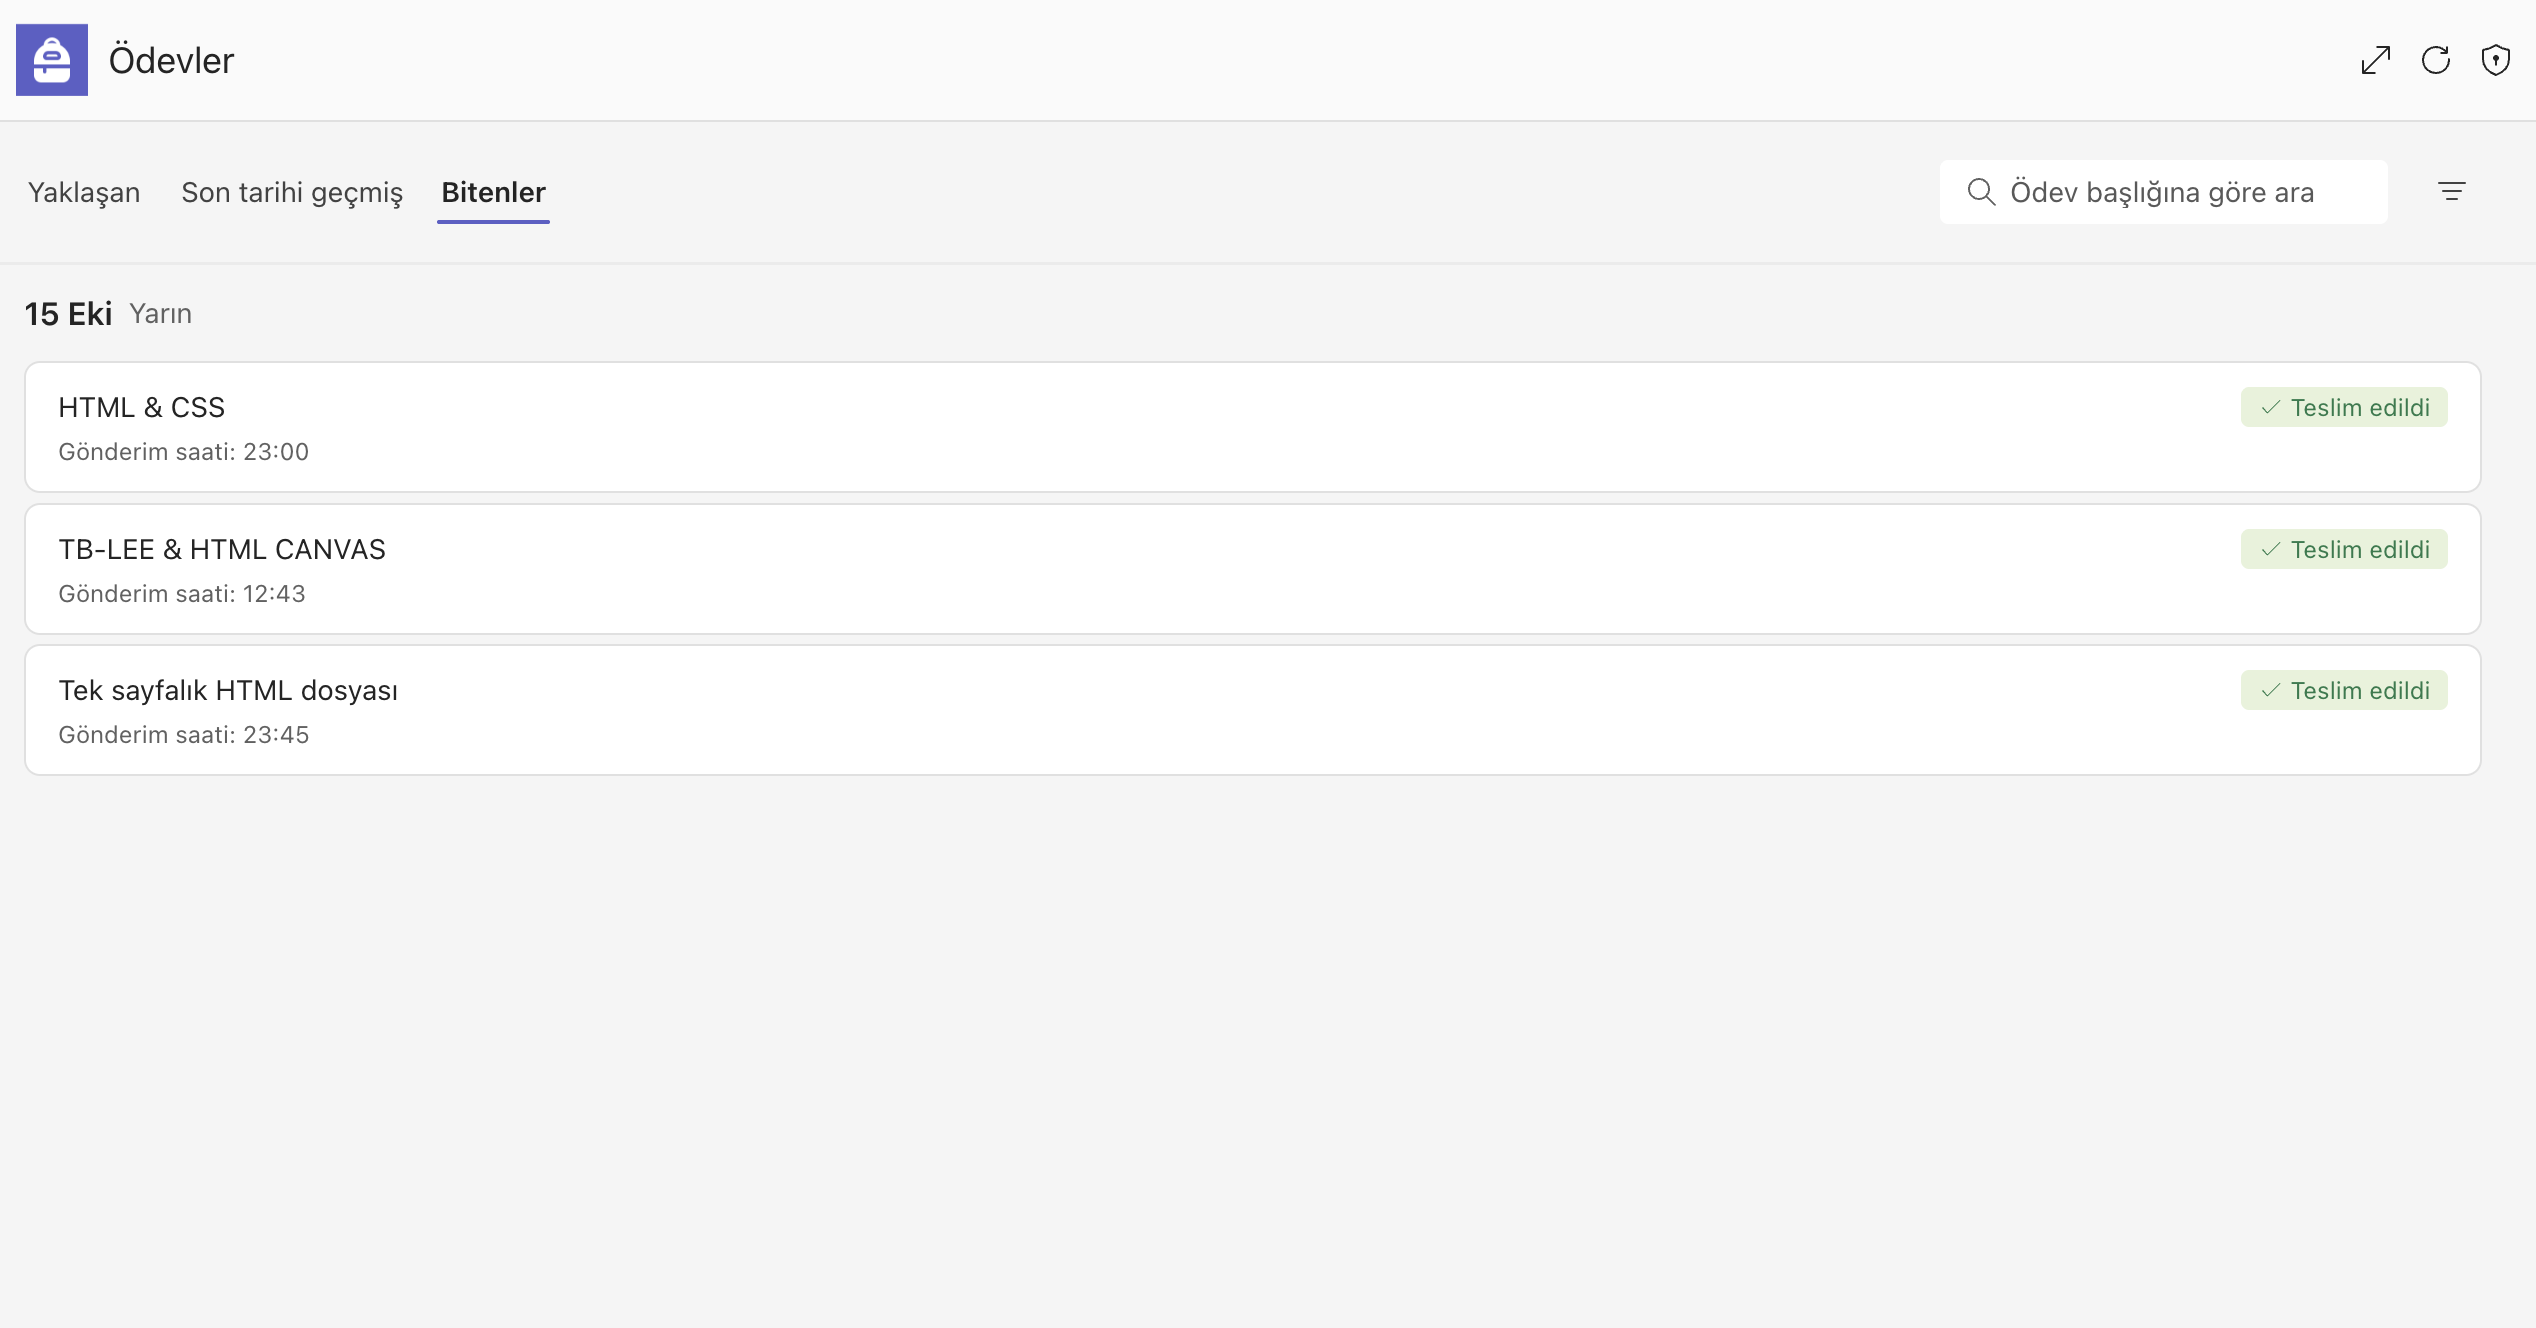
\includegraphics[width=0.9\textwidth]{sureckanit.png}
\section{Ödevler}
\subsection{Ödev 1}
Satır 35  ile 50 arasındaki kod bloğunu kullanarak ödev sayısı kadar subsection oluşturabilirsiniz. Bütün ödevler section 2 içinde sub olarak verilmeli.
\subsubsection{Teslim Edilen Ödevin Görseli}
\includegraphics[width=0.7\textwidth]{odev1.png}

\subsubsection{Süreç Odaklı Sorulara Cevaplar}
\begin{itemize}
  
    \item \textbf{Yöneltilen soruyu ekleyin:} Cevabınız normal yazı olsun.
    \item \textbf{Yöneltilen soruyu ekleyin:} Cevabınız normal yazı olsun.
    \item \textbf{Yöneltilen soruyu ekleyin:} Cevabınız normal yazı olsun.
    \item \textbf{Yöneltilen soruyu ekleyin:} Cevabınız normal yazı olsun.
    \item \textbf{Yöneltilen soruyu ekleyin:} Cevabınız normal yazı olsun.
    \item \textbf{Yöneltilen soruyu ekleyin:} Cevabınız normal yazı olsun.
    \item \textbf{Yöneltilen soruyu ekleyin:} Cevabınız normal yazı olsun.
\end{itemize}



% ----------------------------
\section{Gelişim Odaklı Sorular (Vizeye Özel)}
Dilerseniz subsection'ları silerek cevabınız bir essay formatında buraya yazabilirsiniz.
\subsection{Soru 1}
Cevabınız burada.

\subsection{Soru 2}
Cevabınız burada.

\subsection{Soru 3}
Cevabınız burada.

\subsection{Soru 4}
Cevabınız burada.

\subsection{Soru 5}
Cevabınız burada.

\subsection{Soru 6}
Cevabınız burada.

\subsection{Soru 7}
Cevabınız burada.

% ----------------------------
\section{Katkı Özeti Sayfası}
\textbf{Amaç:} Haftalık çalışmaların Teams üzerindeki paylaşımlarını belgelemek ve toplam katkıyı göstermek. Amaç kısmını silerek essay formatında cevabınızı yazın.
\begin{landscape}
\begin{tabular}{|c|c|c|c|}
\hline
Hafta & Paylaşım Sayısı & Ekran Görüntüleri & Açıklama \\
\hline
1 & 3 & \includegraphics[width=0.2\textwidth]{hafta1-1.png} \includegraphics[width=0.2\textwidth]{hafta1-2.png} \includegraphics[width=0.2\textwidth]{hafta1-3.png} & Kod ve denemeler paylaşıldı \\
\hline
2 & 3 & \includegraphics[width=0.2\textwidth]{hafta2-1.png} \includegraphics[width=0.2\textwidth]{hafta2-2.png} \includegraphics[width=0.2\textwidth]{hafta2-3.png} & Döngü ve etkileşim çalışmaları paylaşıldı \\
\hline
3 & 4 & \includegraphics[width=0.2\textwidth]{hafta3-1.png} \includegraphics[width=0.2\textwidth]{hafta3-2.png} \includegraphics[width=0.2\textwidth]{hafta3-3.png} \includegraphics[width=0.2\textwidth]{hafta3-4.png} & Mini proje denemeleri paylaşıldı \\
\hline
\end{tabular}
\end{landscape}
% ----------------------------
\appendix
\section*{Ek 1 – Resim Ekleme Rehberi}
\addcontentsline{toc}{section}{Ek 1 – Resim Ekleme Rehberi}

\textbf{Bu ek, Overleaf üzerinde LaTeX kullanarak resim ekleme konusunda size yardımcı olmak için hazırlanmıştır. 
Belgeyi teslim etmeden önce bu bölümü siliniz.}

\subsection*{1. Dosya Hazırlığı}
\begin{itemize}
    \item Tüm resim dosyalarınızı Overleaf projenizin sol tarafındaki klasöre yükleyin.
    \item Resim dosyaları \texttt{.png}, \texttt{.jpg}, veya \texttt{.jpeg} formatında olabilir.
    \item Dosya adlarında Türkçe karakter, boşluk veya büyük harf \textbf{kullanmayın.}
    \item Örnek dosya adları: \texttt{odev1.png}, \texttt{hafta2-1.jpg}, \texttt{sureckanit.png}
\end{itemize}

\subsection*{2. Resim Ekleme Komutu}
Bir resmi sayfaya eklemek için şu komutu kullanın:
\begin{verbatim}
\includegraphics[width=0.5\textwidth]{dosyaadi.png}
\end{verbatim}

\begin{itemize}
    \item \texttt{width=} değeri, resmin sayfadaki genişliğini belirler. 
      Örnek: \texttt{0.5\textwidth}  sayfanın yarısı kadar.
    \item Dosya adını uzantısıyla birlikte yazın.
    \item Width ayarlarına metin akışı ve  okunabilirlik açısından dikkat edelim.
\end{itemize}

\subsection*{3. Birden Fazla Resmi Yan Yana Koymak}
Aynı satırda birkaç görsel göstermek için arka arkaya \texttt{\textbackslash includegraphics} komutları yazabilirsiniz:
\begin{verbatim}
\includegraphics[width=0.3\textwidth]{hafta1-1.png}
\includegraphics[width=0.3\textwidth]{hafta1-2.png}
\includegraphics[width=0.3\textwidth]{hafta1-3.png}
\end{verbatim}

\subsection*{4. Sık Karşılaşılan Hatalar}
\begin{itemize}
    \item \textbf{“File not found” hatası:} Dosya adı yanlış yazılmış veya yüklenmemiştir.
    \item \textbf{Resim çok büyük:} \texttt{width} değerini küçültün (\texttt{0.3\textwidth} vb.).
    \item \textbf{Resim görünmüyor:} Dosya uzantısı (\texttt{.png}, \texttt{.jpg}) eklenmemiş olabilir.
\end{itemize}

\subsection*{5. Örnek Uygulama}
Aşağıdaki örnek, tek bir resmin “Ödev 1” alt başlığına nasıl ekleneceğini göstermektedir:
\begin{verbatim}
\subsubsection{Teslim Edilen Ödevin Görseli}
\includegraphics[width=0.5\textwidth]{odev1.png}
\end{verbatim}

\vspace{1cm}
\noindent\rule{\textwidth}{0.4pt}
\textit{Not:
Teslim etmeden önce “Ek 1 – Resim Ekleme Rehberi” bölümünü siliniz.}

\end{document}
